\documentclass[a4paper, 12pt]{article}
% \documentclass[draft, 12pt]{article}
\usepackage[utf8]{inputenc}
\usepackage[brazilian]{babel}
\usepackage{graphicx}
\usepackage{amssymb, mathrsfs, amsfonts, amsmath, esint, relsize, bm}
\usepackage{hyperref}
\usepackage{caption}
\usepackage{indentfirst} 
\usepackage{xcolor}
\usepackage{csquotes} % When using babel or polyglossia with biblatex, loading csquotes is recommended to ensure that quoted texts are typeset according to the rules of your main language.
\usepackage[ruled,vlined]{algorithm2e} % Algorithm
\usepackage{pdfpages} % Include full PDF file

% References
\usepackage[style=ieee]{biblatex}
\addbibresource{refs.bib}

% \usepackage{hhline}
% \usepackage{color}
% \usepackage{soul}
% \usepackage[table,xcdraw]{xcolor}
% \usepackage{enumerate}

%% My commands
% \newcommand{\myref}[1]{{\color{blue} \ref{#1}}} % Display a blue color for linking figures, tables, equations, etc..
% \newcommand{\mywidth}{.6} % Standard for figures
% \hypersetup{linkcolor=blue, filecolor=magenta, urlcolor=cyan}

% Change background color
% \usepackage{pagecolor,lipsum}% http://ctan.org/pkg/{pagecolor,lipsum}

% \definecolor{maroon}{cmyk}{0,0.87,0.68,0.32}

\begin{document}
% \pagecolor{yellow!50!orange} % ``marcador'' de página feita (movimentas ou comentá-lo de acordo com o avanço do trabalho)

%--------------------------------------------------------------------------
% Capa do relatório
\begin{titlepage}
    \begin{center}
        \includegraphics[width=2cm]{adj/brasao.png}\\
        {\large {Universidade Federal do Ceará}}\\
        {\large {Centro de Tecnologia}}\\
        {\large {Departamento de Engenharia de Teleinformática}}\\
        {\large {Sistemas de Comunicações Digitais - TI0069}}
    \end{center}

    \vspace{100pt}
    
    \begin{center}
        {\large \textbf {Trabalho 01: Modulação Digital}}
    \end{center}
    
    \vspace{100pt}
    
    \begin{table}[h]
    \begin{tabular}{ll}
        \textbf{Aluno:}         &       \\
        Lucas de Souza Abdalah  & 385472
    \end{tabular}
    \end{table}
    
    \begin{table}[h]
    \begin{tabular}{l}
        \textbf{Professor:} André Almeida   \\
        \textbf{Data de Entrega do Relatório:} 28/03/2021
    \end{tabular}
    \end{table}
    
    \vspace{\fill}
    
    \begin{center}
        Fortaleza\\
        2021
    \end{center}
    
    \end{titlepage}
    
    %--------------------------------------------------------------------------
    % Sumario do relatorio
    
    \tableofcontents
    \thispagestyle{empty}
    \clearpage

% Exemplo de citação usando \cite{}
%--------------------------------------------------------------------------
% Exemplos
\section*{Exemplos}

% Place holder de texto
% \lipsum[1]

Para referenciar imagens~\ref{fig:brasao_UFC}, tabelas~\ref{tab:frequencia_tensao} e equações~\ref{eq:frequencia_ganho}.

\begin{figure}[!ht]
    \centering
    \includegraphics[width=0.15\textwidth]{adj/brasao.png}
    \caption{Exemplo de como adicionar uma imagem.}
    \label{fig:brasao_UFC}
\end{figure}

\begin{table}[!ht]
    \centering
    \begin{tabular}{|c|c|}
    \hline
    Frequência (Hz) & Tensão Máxima (V) \\ \hline
    0,558            & 12,11            \\ \hline
    2,132            & 11,15            \\ \hline
    4,822            & 8,62             \\ \hline
    \end{tabular}
    \caption{Frequência da onda de entrada e a tensão máxima da saída do circuito integrador.}
    \label{tab:frequencia_tensao}
\end{table}

\begin{equation}
    f_{gu} = A_{VD}\times f_{c}
    \label{eq:frequencia_ganho}
\end{equation}

% Exemplo de citação usando \cite{}
E quando tirar informação de alguma fonte, deve adicionar no formato de bibtex no arquivo refs.bib e por fim citá-los assim:~\cite{Sedra} \cite{Boylestad} \cite{Fonseca}, de modo que a seção de referência é criada e indexada diretamente com estes chamados da função.

\clearpage

\section{Introdução}
% \clearpage

\section{Simulações}
\section{Problema 1 - \texorpdfstring{$M$}{M}-QAM}

Na modulação,\textit{quadrature amplitude modulation} (QAM) os símbolos de informação são mapeados nas amplitudes das portadoras em fase e quadratura. Um modelo simplificado do sinal transmitido é visto como a equação~\ref{eq:QAM_coef}.
\begin{equation}
    s_m(t) = ( A_m^{(\text{real})} + j A_m^{(\text{imag})}) g(t)
    \label{eq:QAM_coef}
\end{equation}

% No caso especial em que amplitudes $A_m^{(\text{real})}$ e $A_m^{(\text{imag})}$ assumem valores discretos no conjunto da equação~\ref{eq:QAM_retangular}, a constelação é chamada QAM retangular. O QAM retangular se aplica ao caso estudado a seguir, pois a quantidade de símbolos utilizados ($M = \{4, 16, 64\}$) se encaixam na condição e é utilizado para construção do alfabeto da modulação~\cite{Cecilio}.
%  A função \href{https://raw.githubusercontent.com/lucasabdalah/Courses-HWs/SCD/Sistemas%20de%20Comunicacoes%20Digitais/matlab/problema1/const_MQAM.m}{const\_MQAM.m} foi

desenvolvida de modo a construir o alfabeto como uma matriz para ordenar os símbolos da esquerda para direita em linhas de símbolos ímpares e, da direita para esquerda em linhas pares.
\begin{equation}
    A_m = \{(2m -\sqrt{M} - 1)d \}_{m=1}^{\sqrt{M}}
    \label{eq:QAM_retangular}
\end{equation}


% -------------------------------------------------------------------
\subsection{Energia da Constelação} 
Para calcular a energia média, é suficiente de calcular a equação~\ref{eq:E_media}, desenvolvida em \cite{Cecilio,Proakis}.
\begin{equation}
    \mathcal{E}_{media} = \frac{M-1}{3} \mathcal{E}_g
    \label{eq:E_media}
\end{equation}
Sendo $g(t)$ o pulso de energia unitária, $\mathcal{E}_g = 1$. O resultado é computado pela função função \href{https://raw.githubusercontent.com/lucasabdalah/Courses-HWs/SCD/Sistemas%20de%20Comunicacoes%20Digitais/matlab/problema1/energia_MQAM.m}{energia\_MQAM.m} para cada constelação QAM e é registrado na Tabela~\ref{tab:Resume_QAM}.

A relação entre $\mathcal{E}_{media} = \mathcal{E}_b \log_2{M}$ permite calcular diretamente a energia média de bit ($\mathcal{E}_b$), resultando na equação~\ref{eq:E_b}
\begin{equation}
    \mathcal{E}_b = \frac{M-1}{3\log_2 M} \mathcal{E}_{media}
    \label{eq:E_b}
\end{equation}

% -------------------------------------------------------------------
\subsection{Distância Mínima entre Símbolos}
O parâmetro $d$ é a distância entre os símbolos adjacentes, e pode ser obtido com o cálculo da distância euclidiana entre estes, como na equação~\ref{eq:parametro_d}.

\begin{equation}
    \begin{split}
        d & = \sqrt{\frac{\mathcal{E}_g}{2}[(A_{mi} - A_{ni})^2 + (A_{mq} - A_{nq})^2]}\\
        & = \sqrt{\frac{3 \mathcal{E}_{media}}{2(M-1)}}
    \end{split}
    \label{eq:parametro_d}
\end{equation}

Essa distância é computada pela função \href{https://raw.githubusercontent.com/lucasabdalah/Courses-HWs/SCD/Sistemas%20de%20Comunicacoes%20Digitais/matlab/problema1/d_MQAM.m}{d\_MQAM.m} e registrada na Tabela~\ref{tab:Resume_QAM}.

\begin{table}[!ht]
    \centering
    \begin{tabular}{|c|c|c|c|}
        \hline
        $M$-QAM & $\mathcal{E}_{media}$ & $\mathcal{E}_{b}$ & $d$ \\ \hline
        & &  &  \\ 
        $M$ & $\frac{M-1}{3} \mathcal{E}_g$ & $ \frac{M-1}{3\log_2 M} \mathcal{E}_g$ & $\sqrt{\frac{3 \mathcal{E}_{media}}{2(M-1)}} $ \\ 
         &   &   &  \\ \hline
        $4$  & 1 & $1.67\times 10^{-1}$ & $\sqrt{2}/2$\\ \hline
        $16$ & 5 & $4.67\times 10^{-1}$ & $\sqrt{2}/2$\\ \hline
        $64$ & 21 & $1.17\times 10^{0}$ & $\sqrt{2}/2$\\ \hline
    \end{tabular}
    \caption{Informações gerais calculadas para a modulação $M$-QAM.}
    \label{tab:Resume_QAM}
\end{table}

% -------------------------------------------------------------------
\subsection{Modulador (Codificação de Gray)}
O mapeador da constelação $M$-QAM consiste em uma função  que recebe uma sequência de bits e retorna o símbolo equivalente: \href{https://raw.githubusercontent.com/lucasabdalah/Courses-HWs/SCD/Sistemas%20de%20Comunicacoes%20Digitais/matlab/problema1/mapping_MQAM.m}{mapping\_MQAM.m}. Dentro desta função, é criado um alfabeto de código binário e na convertido em Gray. \href{https://raw.githubusercontent.com/lucasabdalah/Courses-HWs/SCD/Sistemas%20de%20Comunicacoes%20Digitais/matlab/gray_const.m}{gray\_const.m} 

Esta codificação é baseada em um algoritmo recursivo~\ref{alg:Gray}, cujo recebe uma sequência de bits orientadas pelo bit mais importante (MSB)~\cite{Gray}. A recursão está na operação ``ou exlusivo'' (\textit{xor}), denotada pelo símbolo $(\otimes)$. Este cálculo é executado na função \href{https://raw.githubusercontent.com/lucasabdalah/Courses-HWs/SCD/Sistemas%20de%20Comunicacoes%20Digitais/matlab/mybin2gray.m}{mybin2gray.m}.

% global change
\SetKwInput{KwData}{Entrada}
\SetKwInput{KwResult}{Saída}

\begin{algorithm}[!ht]
    \SetAlgoLined
    \KwData{Sequência de Bits $(b)$ - MSB}
    \KwResult{Sequencia em Código Gray $(g)$ - LSB}
    $n = 0$\;
    $K = \text{length}(b)$\;
    \While{$K > n$}{
        \eIf{$K==n$}
        {$g_{(K-n)} = b_{(K-n)}$ \;}
        {$g_{(K-n)} = b_{(K-n+1)} \otimes b_{(K-n)}$\;}
        $n=n+1$;\;}
    $g = flip(g)$\;
    \caption{Codificação de Gray}
    \label{alg:Gray}
\end{algorithm}

\clearpage

A~\ref{tab:Alfabeto_Gray} mostra um exemplo de conversão para código Gray de uma sequência de 2 bits. Seguindo o mesmo procedimento um alfabeto de qualquer tamanho pode ser criado.

\begin{table}[!ht]
    \centering
    \begin{tabular}{|c|c|c|c|}
        \hline
        Decimal & Binário & Gray & Decimal \\ \hline
        0 & 00 & 00 & 0\\ \hline
        1 & 01 & 01 & 1\\ \hline
        2 & 10 & 11 & 3\\ \hline
        3 & 11 & 10 & 2\\ \hline
    \end{tabular}
    \caption{Tabela de tradução de binário para Gray com 2 bits.}
    \label{tab:Alfabeto_Gray}
\end{table}

As constalações $M$-QAM para $M = \{4, 16, 64\}$ são apresentadas nas figuras~\ref{fig:4_QAM_plot}, \ref{fig:16_QAM_plot} e \ref{fig:64_QAM_plot}, respectivamente. É possível observar os valores dos símbolos em fase e quadratura, além do equivalente em binário.

\begin{figure}[!ht]
    \centering
    \includegraphics[width=1.0\textwidth,clip=true,trim={1.5cm 8.5cm 1.8cm 8.3cm}]{C:/Users/lukin/Documents/GitHub/Courses-HWs/Sistemas de Comunicacoes Digitais/matlab/problema1/fig/4_QAM_plot.pdf}
    \caption{Constelação 4-QAM plot.}
    \label{fig:4_QAM_plot}
\end{figure}

\clearpage

\begin{figure}[!ht]
    \centering
    \includegraphics[width=1.0\textwidth,clip=true,trim={1.5cm 8.5cm 1.8cm 8.3cm}]{C:/Users/lukin/Documents/GitHub/Courses-HWs/Sistemas de Comunicacoes Digitais/matlab/problema1/fig/16_QAM_plot.pdf}
    \caption{Constelação 16-QAM plot.}
    \label{fig:16_QAM_plot}
\end{figure}

\begin{figure}[!ht]
    \centering
    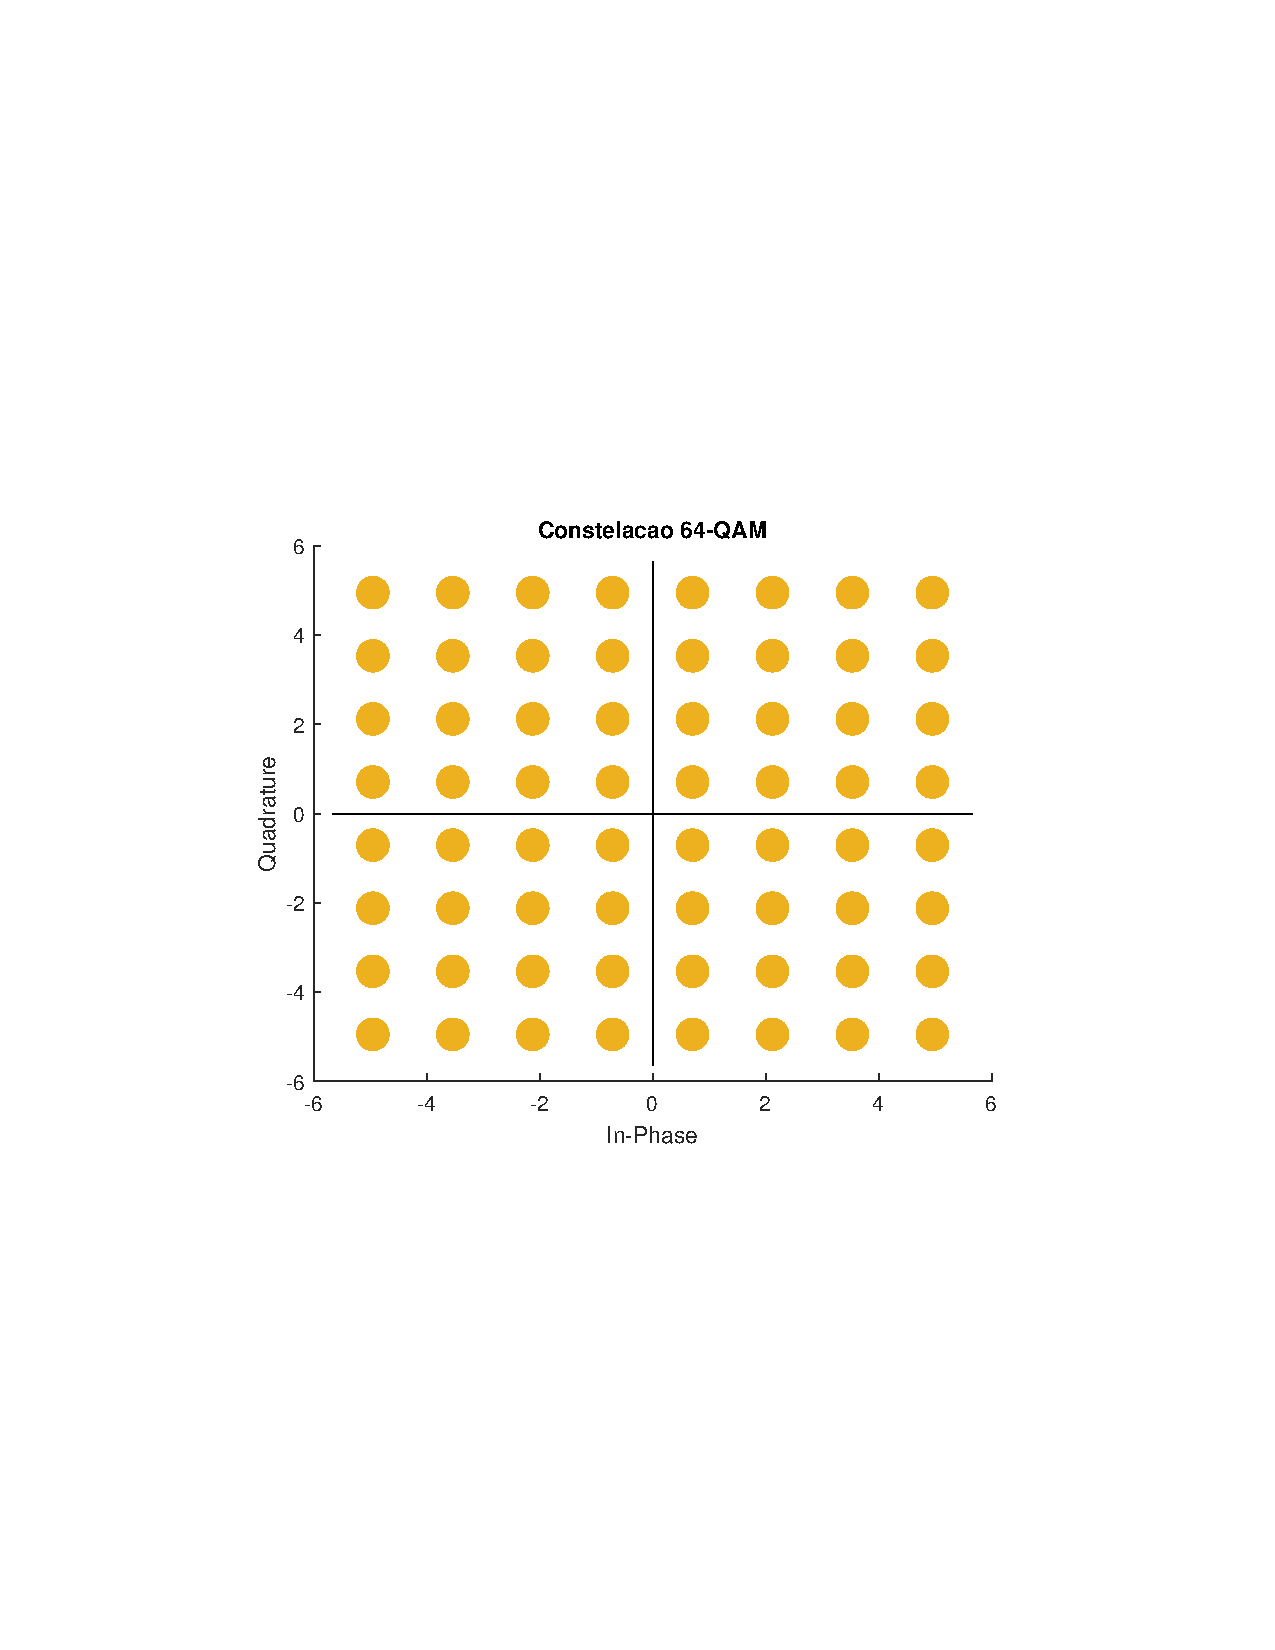
\includegraphics[width=1.0\textwidth,clip=true,trim={1.5cm 8.5cm 1.8cm 8.3cm}]{C:/Users/lukin/Documents/GitHub/Courses-HWs/Sistemas de Comunicacoes Digitais/matlab/problema1/fig/64_QAM_plot.pdf}
    \caption{Constelação 64-QAM plot.}
    \label{fig:64_QAM_plot}
\end{figure}

\clearpage

% -------------------------------------------------------------------
\subsection{Demodulador}

A função que decodifica um símbolo tem como entrada o próprio símbolo: $A_n^{(\text{real})}$ e $A_n^{(\text{imag})}$, $M$ e $d$. 

O alfabeto da constelação $M$-QAM é gerada e uma vez estes definidos, a área de decisão é desenhada a partir em função de $M$ e $d$. Basicamente, o símbolo selecionado é aquele que minimiza a distância euclidiana entre o símbolo recebido e o do alfabeto, como mostra a equação~\ref{eq:dist_eucliadiana}.
\begin{equation}
    d_{mn} = \sqrt{|| s_m - s_n||^2}
    \label{eq:dist_eucliadiana}
\end{equation}

A função que executa estes comando é a \href{https://raw.githubusercontent.com/lucasabdalah/Courses-HWs/SCD/Sistemas%20de%20Comunicacoes%20Digitais/matlab/problema1/demapping_MQAM.m}{demapping\_MQAM.m} e ela retorna o símbolo decodificado e os bits equivalente do alfabeto de Gray. 

As figuras~\ref{fig:4_QAM_d_E} e \ref{fig:16_QAM_d_E} mostram uma geração de sequência de 50 símbolos aleatórios (\textit{i.i.d}) passando pelo demodulador com o traçado da distância euclidiana entre o símbolo recebido e o equivalente escolhido na constelação.

\begin{figure}[!ht]
    \centering
    \includegraphics[width=1.0\textwidth,clip=true,trim={1.5cm 8.5cm 1.8cm 8.3cm}]{C:/Users/lukin/Documents/GitHub/Courses-HWs/Sistemas de Comunicacoes Digitais/matlab/problema1/fig/4example_QAM_plot.pdf}
    \caption{Exemplo de 4-QAM plot.}
    \label{fig:4_QAM_d_E}
\end{figure}

\clearpage 

\begin{figure}[!ht]
    \centering
    \includegraphics[width=1.0\textwidth,clip=true,trim={1.5cm 8.5cm 1.8cm 8.3cm}]{C:/Users/lukin/Documents/GitHub/Courses-HWs/Sistemas de Comunicacoes Digitais/matlab/problema1/fig/16example_QAM_plot.pdf}
    \caption{Exemplo de 16-QAM plot.}
    \label{fig:16_QAM_d_E}
\end{figure}
\clearpage
\section{Problema 2 - Probabilidade de Erro: \texorpdfstring{$M$}{M}-QAM}
Para calcular a probabilidade de erro $P(e)$ de cada constelação~\ref{eq:Pe_M_QAM} é necessário computar a energia da cosnstelação e do ruído, respectivamente, $E_s$ e $N_o$, que é desenvolvida em~\cite{Cecilio}. A função~\href{https://raw.githubusercontent.com/lucasabdalah/Courses-HWs/SCD/Sistemas%20de%20Comunicacoes%20Digitais/matlab/problema2/Pe_MQAM.m}{Pe\_MQAM.m} é utlizada para calcular a probabilidade de erro.
\begin{equation}
    P(e) = 4 \left(1-\frac{1}{\sqrt{M}}\right) Q\left(\sqrt{\frac{3}{M-1}\frac{E_s}{N_0}}\right) - 4\left(1-\frac{1}{\sqrt{M}}\right)^2 Q^2\left(\sqrt{\frac{3}{M-1}\frac{E_s}{N_0}}\right)
    \label{eq:Pe_M_QAM}
\end{equation}

Para valores mais elevados de relação sinal-ruído(\textit{SNR}), a equação~\ref{eq:Pe_M_QAM} pode ser reduzida para~\ref{eq:Pe_reduzida_M_QAM}, pois o segundo termo ao quadrado se torna irrelevante.
\begin{equation}
    P(e) = 4 \left(1-\frac{1}{\sqrt{M}}\right) Q\left(\sqrt{\frac{3}{M-1}\frac{E_s}{N_0}}\right)
    \label{eq:Pe_reduzida_M_QAM}
\end{equation}

\begin{figure}[!ht]
    \centering
    \includegraphics[width=1.0\textwidth,clip=true,trim={1.5cm 8.5cm 1.8cm 8.3cm}]{C:/Users/lukin/Documents/GitHub/Courses-HWs/Sistemas de Comunicacoes Digitais/matlab/problema2/fig/Erro_Teorico_MQAM.pdf}
    \caption{Probabilidade de erro $(P(e))$ teórico $M$-QAM.}
    \label{fig:Erro_Teorico_MQAM}
\end{figure}

Nas simulações realizadas, os resultados são semelhantes, além de reduzir o custo computacional.

Entretanto, para manter uma fidedignidade dos resultados o gráfico mostrado na figura~\ref{fig:Erro_Teorico_MQAM} a probabilidade $P(e)$ é caculada a partir da equação completa~\ref{eq:Pe_M_QAM}, variando a \textit{SNR} de 0:2:20 dB.
\clearpage
\section{Problema 3 - Canal RAGB: \texorpdfstring{$M$}{M}-QAM}

Considerando que um sinal ($s_m$) de mensagem passa por um canal de Ruído Adivitivo Gaussiano Branco (RAGB), um modelo como uma variável aleatoria Gaussiana complexa, como na equação~\ref{fig:4QAM_25dB}. O sinal foi recebeido no filtro casado e é dado por

\begin{figure}[!ht]
    \centering
    \includegraphics[width=1.0\textwidth,clip=true,trim={1.5cm 8.5cm 1.8cm 8.3cm}]{C:/Users/lukin/Documents/GitHub/Courses-HWs/Sistemas de Comunicacoes Digitais/matlab/problema3/fig/4QAM_25dB.pdf}
    \caption{Simulação de transmissão $4$-QAM, com \textit{SNR} de 25dB.}
    \label{fig:4QAM_25dB}
\end{figure}

Para o caso de $16$-QAM

\begin{figure}[!ht]
    \centering
    \includegraphics[width=1.0\textwidth,clip=true,trim={1.5cm 8.5cm 1.8cm 8.3cm}]{C:/Users/lukin/Documents/GitHub/Courses-HWs/Sistemas de Comunicacoes Digitais/matlab/problema3/fig/16QAM_25dB.pdf}
    \caption{Simulação de transmissão $16$-QAM, com \textit{SNR} de 25dB.}
    \label{fig:16QAM_25dB}
\end{figure}

\begin{figure}[!ht]
    \centering
    \includegraphics[width=1.0\textwidth,clip=true,trim={1.5cm 8.5cm 1.8cm 8.3cm}]{C:/Users/lukin/Documents/GitHub/Courses-HWs/Sistemas de Comunicacoes Digitais/matlab/problema3/fig/64QAM_25dB.pdf}
    \caption{Simulação de transmissão $64$-QAM, com \textit{SNR} de 25dB.}
    \label{fig:64QAM_25dB}
\end{figure}


\begin{figure}[!ht]
    \centering
    \includegraphics[width=1.0\textwidth,clip=true,trim={1.5cm 8.5cm 1.8cm 8.3cm}]{C:/Users/lukin/Documents/GitHub/Courses-HWs/Sistemas de Comunicacoes Digitais/matlab/problema3/fig/Erro_teoricaxAWGN_MQAM.pdf}
    \caption{Probabilidade teórica de erro vs. simulação de transmissão $M$-QAM em canal RAGB.}
    \label{fig:Erro_teoricaxAWGN_MQAM}
\end{figure}


\section{Conclusão e Resultados}

\clearpage

% Bibliografia
% LateX vai gerar as ``Referências'' automaticamente
% usando a função \cite{nome} do pacote BibTeX é possível
% "puxar todas as informações do arquivo 'refs.bib'
% O nome do arquivo é o primeiro parâmetro de cada referência
% Um exemplo esta é utilizado na primeira seção
% \AtNextBibliography{\small}             % To set a smaller font size for bibliography
\printbibliography[heading=bibintoc]    % Print the references

\end{document}